
\documentclass[letterpaper, 10 pt, conference]{ieeeconf}  % Comment this line out if you need a4paper
\IEEEoverridecommandlockouts                              % This command is only needed if 
                                                          % you want to use the \thanks command
\overrideIEEEmargins                                      % Needed to meet printer requirements.


% Bibliography
\usepackage{biblatex}
\addbibresource{references.bib}

% Math
\usepackage{physics}
\usepackage{siunitx}
\sisetup{output-exponent-marker=\ensuremath{\mathrm{e}}}
\usepackage{amsmath}
\usepackage{amsfonts}
\usepackage{amssymb}

% Optimization and Algorithms
\usepackage{optidef}
\usepackage{algorithmicx}
\usepackage{algorithm,algpseudocode}

% Formatting
\usepackage{xcolor}
\usepackage{bm}  % for bold symbols 
\usepackage{booktabs}  % better tables
\usepackage{pifont}  % for x mark
\usepackage{graphicx}
\usepackage{hyperref}

% Plotting
\usepackage{pgfplots}
\pgfplotsset{compat=1.15,
	legend style={font=\footnotesize},
}
\usepackage{tikzscale}

% Custom commands
\newcommand{\half}{\frac{1}{2}}
\newcommand{\R}{\mathbb{R}}
\newcommand{\Q}{\mathbb{S}^3}
\newcommand{\skewmat}[1]{[#1]^\times}

\newcommand{\rmap}{\varphi}
\newcommand{\invrmap}{\varphi^{-1}}

\newcommand{\dR}{\delta \mathcal{R}}
\newcommand{\rot}{ \mathcal{R} }
\newcommand{\dq}{\delta q}
\newcommand{\q}{\textbf{q}}
\newcommand{\eq}{_\text{eq}}
\newcommand{\traj}[2][N]{#2_{0:{#1}}}
\newcommand{\pass}{{\color{green} \checkmark}}
\newcommand{\fail}{{\color{red} \ding{55}}}

\newcommand{\todo}[1]{\textcolor{red}{TODO: #1}}


\title{\LARGE \bf
Planning with Attitude
}

\author{Brian Jackson$^1$ and Zachary Manchester$^1$%
    \thanks{
        $^1$Robotics Institute, 
        Carnegie Mellon University, 
        5000 Forbes Ave, Pittsburgh, PA, USA
    }
}

\begin{document}
\maketitle

% Planning and controlling trajectories for floating-base robotic systems that
% experience large attitude changes is challenging due to the nontrivial group
% structure of 3D rotations. This paper introduces a powerful, computationally
% efficient, and accessible approach for adapting existing Newton and
% gradient-based methods to correctly account for the group structure of
% rotations. We demonstrate the effectiveness of the approach by modifying the
% ALTRO solver to optimize a loop-de-loop trajectory for a quadrotor, enabling
% the solver to find a dramatically better solution in less than a third the
% time.

\section{INTRODUCTION} 

    Many robotic systems---including quadrotors, airplanes, satellites, 
    underwater vehicles, and quadrupeds---can perform arbitrarily large three-dimensional
    translations and rotations as part of their normal operation. While simply
    representing the attitude of these sytems is nontrivial, generating and tracking
    motion plans for floating-base systems is an even more challenging problem.

    Many approaches have been taken to address the problem of motion planning and control
    on the space of rigid body motions \cite{Kobilarov2011, Saccon2013,
    watterson2020control}; most of these rely heavily on ideas and notation from
    differential geometry. Despite some impressive results, many of these ideas have not
    been widely adopted by the robotics community, and many practitioners continue to
    ignore the group structure of rotations. One issue preventing wider adoption is that
    accounting for this structure requires low-level changes to the underlying
    optimization algorithms, which is difficult or impossible when relying on existing
    off-the-shelf solvers.
    
    % \todo{I'm worried that SE(3) and SO(3) results are getting confused/conflated here. I
    % would explicitly talk about both, emphasize that we're handling SO(3) with the
    % quaternion stuff, and that $SE(3) = SO(3) \times \mathbb{R}^3$ is a straightforward
    % extension.}

    To address this lack of solver support, we formulate a straightforward, generic
    method for adapting existing Newton and gradient-based algorithms to correctly
    account for the group structure of rotations. Based entirely on basic mathematical
    tools from linear algebra and calculus, our method is computationally efficient and
    should be both accessible and familiar to most roboticists. We apply this method to
    the ALTRO solver \cite{howell2019altro} and demonstrate its performance on a 
    constrained trajectory optimization problem.

\section{Notation and Convensions}

    We begin by defining some useful conventions and notation. 
    Attitude is defined as the rotation from the robot's body frame to a global inertial 
        frame. 
    We also define gradients to be row vectors, that is, for 
        $f(x) : \R^n \to \R$, $\pdv{f}{x} \in \R^{1\times n}$.

    We represent---following the Hamilton convention---a quaternion $\q \in \mathbb{H}$
    as a standard vector $q \in \R^4 := [q_s \;\; q_v^T]^T$ where $q_s \in \R$ and $q_v
    \in \R^3$ are the scalar and vector part of the quaternion, respectively. We denote
    the composition of two quaternions as $\q_3 = \q_2 \otimes \q_1$. We use
    $\skewmat{x}$ to denote the skew-symmetric matrix such that $\skewmat{x} y = x \times
    y$.
        
    \begin{figure}
        \centering
        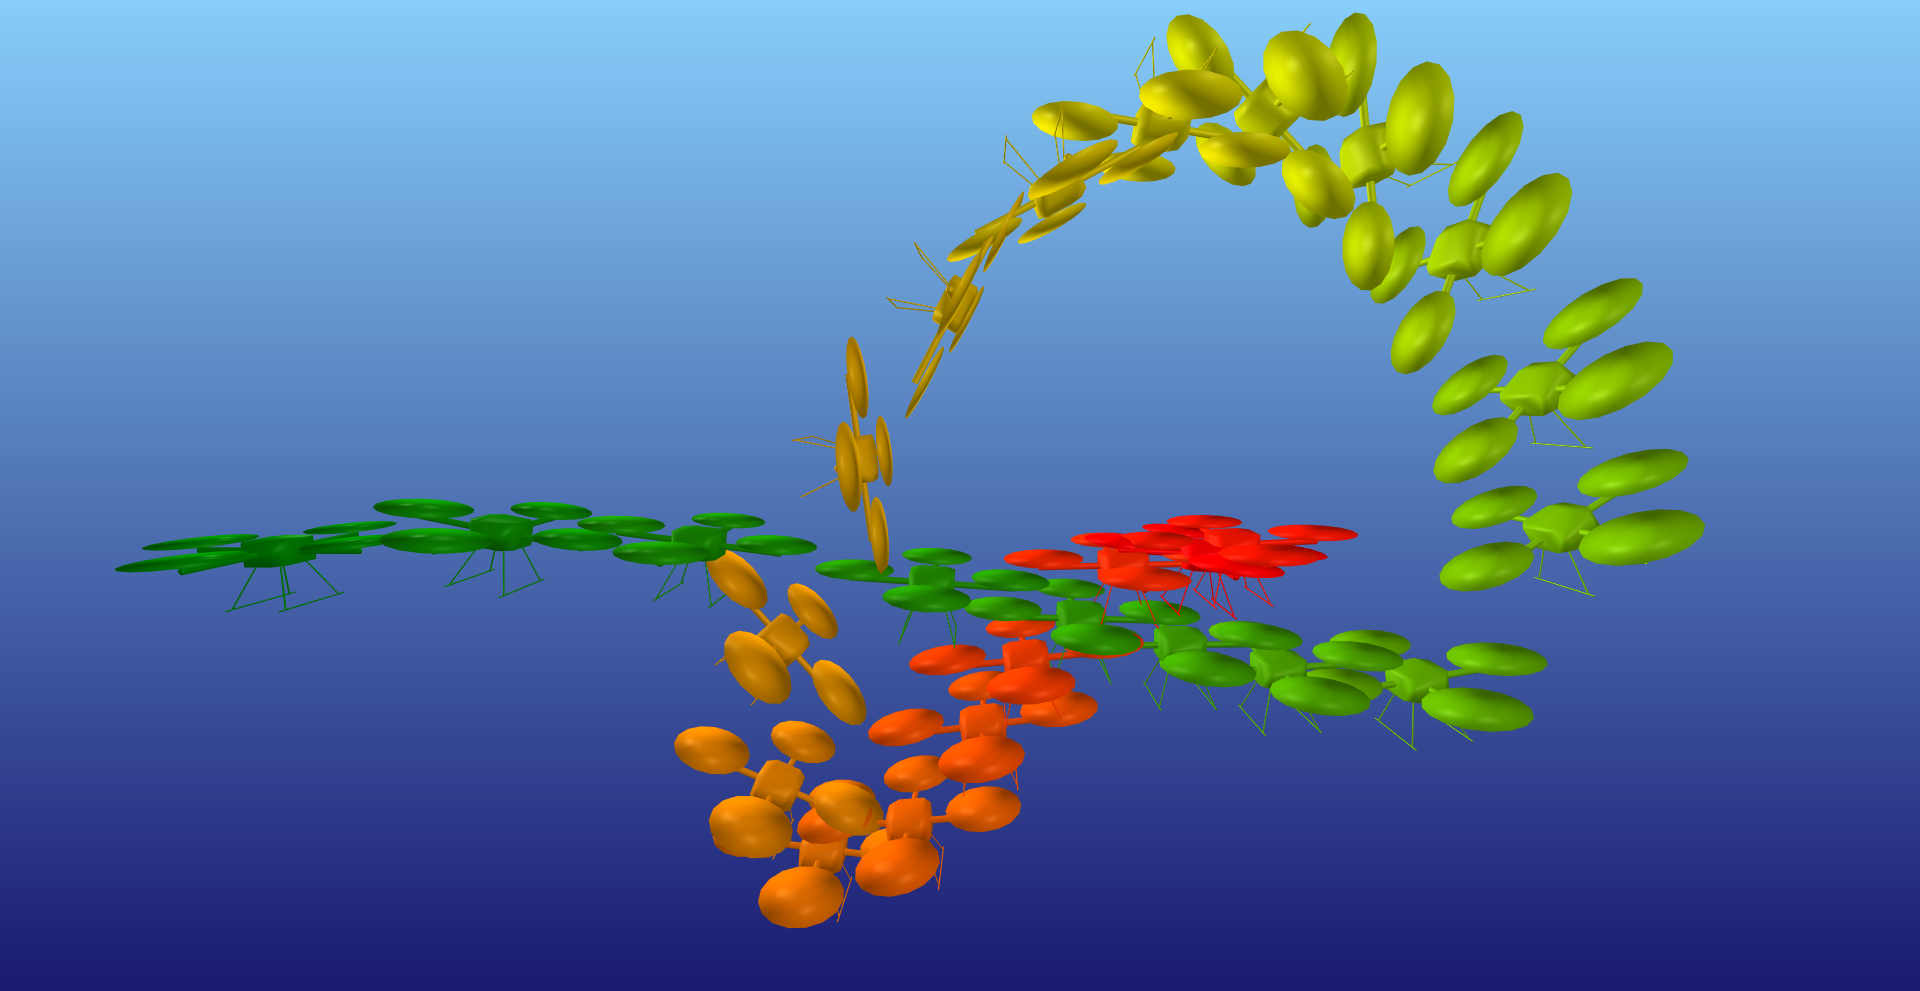
\includegraphics[width=\columnwidth]{figures/quadflip.png}
        \label{fig:quadflip}
        \caption{Snapshots of quadrotor flip trajectory solved using a modified version
        of ALTRO that correctly accounts for the group structure of rotations. These
        modifications make it easier to find trajectories that undergo large changes in
        attitude, such as the loop-de-loop shown here.}
    \end{figure}

\section{Quaternion Differential Calculus} \label{sec:Quaternion_Calculus}
    Most modern methods for planning and control require derivatives with respect to the
    state vector. We present a simple but powerful method for taking derivatives of
    quaternion-valued state vectors. The extension of this method to more general state
    vectors that contain Cartesian products of $SO(3)$, $SE(3)$, and $\mathbb{R}^n$ is
    straightforward.

    The key idea of this section is that differential quaternions live in
    three-dimensional space instead of the four-dimensional space of quaternions; this
    idea should match our intuition given rotations are inherently three-dimensional and
    differential rotations should live in the same space as angular velocities, i.e.
    $\R^3$.

    % \begin{figure}
    %     \centering
    %     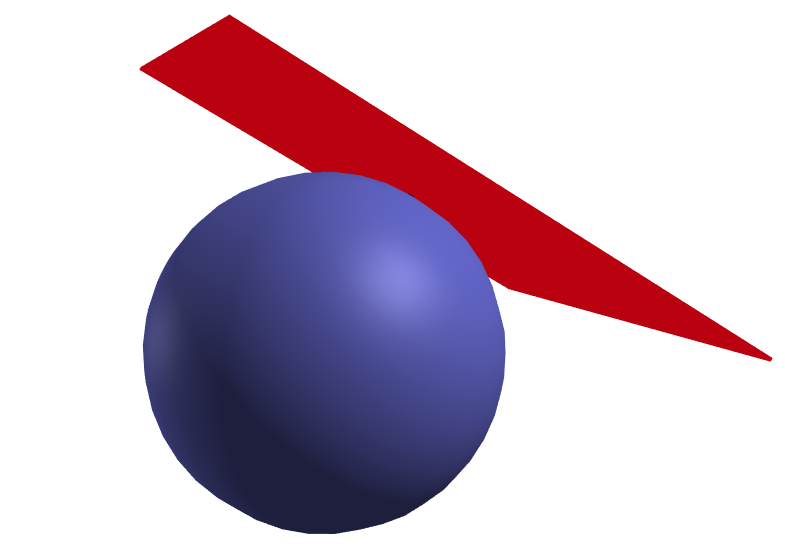
\includegraphics[height=5cm]{figures/tangent_plane.tikz}
    %     \caption{
    %         When linearizing about a point $q$ on an sphere $\mathbb{S}^{n-1}$ in 
    %         n-dimensional space, the tangent space $T$ is a hyper-plane $\R^{n-1}$, 
    %         illustrated here with $n=3$. Therefore, when linearizing about a unit 
    %         quaternion $q \in \Q$, the space of differential rotations lives in $\R^3$.
    %     }
    %     \label{fig:tangent_plane}
    % \end{figure}
    In practice, we have found Rodrigues Parameters to be a very effective representation
    for three-dimensional differential rotations since they are computionally efficient
    and do not inherit the sign ambiguity of quaternions.
    
    The mapping between a vector of Rodrigues parameters $\phi \in \R^3$ and a unit
    quaternion $q$ is known as the Cayley map:
    \begin{equation} \label{eq:cayley}
        q = \varphi(\phi) = \frac{1}{\sqrt{1 + \norm{\phi}^2}} \begin{bmatrix} 1 \\ \phi \end{bmatrix}.
    \end{equation}
    We will also make use of the inverse Cayley map:
    \begin{equation} \label{eq:invcayley}
        \phi = \varphi^{-1}(q) = \frac{q_v}{q_s}.
    \end{equation}

    \subsection{Jacobian of Vector-Valued Functions}
        When taking derivatives with respect to quaternions, we must take into account
        both the composition rule and the nonlinear mapping between the space of unit
        quaternions and our chosen three-parameter error representation.

        Let $\phi \in \R^3$ be a differential rotation applied to a function with
        unit quaternion inputs $y = h(q): \Q \to \R^p$, such that
        \begin{equation} \label{eq:vector_function}
            y + \delta y = h(q \otimes \varphi(\phi)) \approx h(q) +  \nabla h(q) \phi.
        \end{equation}
        We can calculate the Jacobian $\nabla h(q) \in \R^{p \times 3}$ by
        differentiating \eqref{eq:vector_function} with respect to $\phi$, evaluated at
        $\phi = 0$:
        \begin{equation} \label{eq:quat_gradient}
            \nabla h(q) = \pdv{h}{q} \begin{bmatrix} 
                            -q_v^T \\ 
                            q_s I_3 + \skewmat{q_v}
                        \end{bmatrix}
                        := \pdv{h}{q} G(q) 
        \end{equation}
        where $G(q) \in \R^{4 \times 3}$ is referred to as the \textit{attitude Jacobian}, which
        essentially becomes a ``conversion factor'' allowing us to apply results from
        standard vector calculus to the space of unit quaternions. This form is
        particularly useful in practice since $\pdv*{h}{q} \in \R^{p \times 4}$ can be
        obtained using finite difference or automatic differentiation.
        As an aside, although we have used Rodrigues parameters, $G(q)$ is actually the
        same (up to a constant scaling factor) for any choice of three-parameter attitude
        representation.

    \subsection{Other derivatives}
        Using similar techniques, we find useful expressions for the Hessian of a
        scalar-valued function (i.e. $p = 1$):
	    \begin{equation} \label{eq:quat_hessian}
            \nabla^2 h(q) = G(q)^T \pdv[2]{h}{q} G(q) + I_3 \pdv{h}{q}q,
        \end{equation}
        and the Jacobian of a quaternion-valued function $q' = f(q) : \Q \to \Q$:
        \begin{equation} \label{eq:quat_jacobian}
            \nabla f(q) = G(q')^T \pdv{f}{q} G(q).
        \end{equation}


\section{Fast Constrained Trajectory Optimization with Attitude States}
    \subsection{Algorithmic Modifications}
    Here we briefly outline the changes to the ALTRO solver \cite{howell2019altro} to 
    efficiently solve trajectory optimization problems for systems with 3D rotations in the
    state vector. 

    The linearization of the nonlinear discrete dynamics function $x_{k+1} = f(x_k,u_k)$
    is ``corrected'' using \ref{eq:quat_jacobian}: \begin{equation} A = E(f(x,u))^T
    \pdv{f}{x} E(x); \quad B = E(f(x,u))^T \pdv{f}{u}. \end{equation} Here we define the
    \textit{state attitude Jacobian} $E(x)$ to be a block-diagonal matrix where the block
    is an identity matrix for any vector-valued state and $G(q)$ for any quaternion in
    the state vector. Using \eqref{eq:quat_gradient}, \eqref{eq:quat_hessian},
    \eqref{eq:quat_jacobian} we can derive similar modifications to the expansions of the
    cost and constraint functions. We refer the reader to the original ALTRO paper
    \cite{howell2019altro} for futher details on the algorithm.

    These adjustments effectively modify the optimization so that it is performed on 
    differential rotations (or Rodrigues Parameters) instead of the space of unit
    quaternions. In practice, this is analagous to the Multiplicative Extended Kalman
    Filter \cite{markley2014fundamentals} in the state estimation community.

    The iLQR algorithm derives a locally-optimal feedback policy of the form $\delta u =
    K \delta x + d$ during the ``backward pass'' of each iteration, which is then used to
    simulate the system forward during the ``forward pass''. Instead of computing $\delta
    x$ using simple substraction as we would in the original algorithm, we now compute the
    error using the inverse Cayley map \eqref{eq:invcayley} for the quaternion states. The
    rest of the forward pass is unmodified.

    \subsection{Examples}
        To demonstrate the effectiveness of the proposed approach, we tested the modified
        version of ALTRO by solving for a quadrotor flip trajectory (see Figure \ref{fig:quadflip}).
        Four soft ``waypoint'' costs were placed along the trajectory, encouraging the
        quadrotor to follow a loop. The trajectory was initialized with hover controls and a
        state trajectory that smoothly rotated the quadrotor one full rotation about the 
        x-axis while moving to the goal. 
        The modified version of ALTRO solved the problem in 140 ms and 22 iterations, while
        the original version that na\"ively treated the quaternion as a vector in $\R^4$ 
        solved in 420 ms and 58 iterations. The original version failed to provide a nice,
        smooth loop and instead reversed direction halfway through the loop.

        It's also worthwhile to note that this problem cannot be solved as-is with any
        three-parameter representation because of the singularities that occur at 90, 180,
        and 360 degrees for Euler angles, Rodrigues parameters, and MRP's, respectively.
        % A classic approach to overcome this issue is to do discrete switching of the 
        % reference orientation, which requires previous knowledge of the topology of the
        % optimal solution. 
        % \begin{figure}
        %     \centering
        %     \includegraphics[height=4cm, width=8cm]{figures/timing_chart.tikz}
        %     \caption{Timing results for the airplane barrell roll, quadrotor flip, and
        %     quadrotor zig-zag examples using iLQR with roll-pitch-yaw Euler angles (RPY),
        %     quaternions, and the current method. The timing result for the Quadrotor flip
        %     with Euler angles is omitted since it failed to converge.
        %     }
        %     \label{fig:timing_chart}
        % \end{figure}
        
        % \todo{It would be great to compare to both the minimal iLQR stuff and SNOPT or IPOPT with quaternion norm constraints + slack variables (referred to as the ``embedding approach'').}

\section{Conclusion} 

    We have proposed a general, accessible, and computationally efficient approach to
    doing planning and control for systems with one or more unit quaternions in their
    state vectors. The approach allows for straightforward adaptation of many
    gradient and Newton-based methods for optimal control and motion planning, which we demonstrated
    on the ALTRO solver. By exploiting the unique structure of both the trajectory
    optimization problem and the rotation group, the newly modified version of ALTRO will
    likely be able to solve more challenging problems with performance.
    Future work will extend these ideas to Newton-based methods such as direct
    collocation and other domains outside of trajectory optimization.
        

\printbibliography

\end{document}